\chapter{TENSORES DE INÉRCIA DO PROTÓTIPO}
\label{chapter:inercia}

Este capítulo apresenta o cálculo da massa, do centro de massa e do tensor de inércia de cada peça do robô e do conjunto montado. Todos os cálculos seguem o procedimento da Seção \ref{sec:composicao}: cada peça é decomposta em sólidos homogêneos elementares (paralelepípedos e cilindros), cujos tensores no centro de massa são conhecidos (Equações \ref{eq:Ipar} e \ref{eq:Icil}); esses tensores são girados para o sistema da peça e transportados para o centro de massa do conjunto pelo teorema dos eixos paralelos (Equação \ref{eq:steiner}). Os cálculos foram implementados em Python com a biblioteca SymPy, e as massas parciais das peças de madeira foram distribuídas proporcionalmente ao volume (ou, para barras de mesma seção, ao comprimento), supondo densidade uniforme. Os valores de tensor estão expressos em g$\cdot$mm$^2$ (1 g$\cdot$mm$^2 = 10^{-9}$ kg$\cdot$m$^2$) e as posições em mm.

\section{Convenções de Eixos}
\label{sec:eixos}

Cada peça é descrita em um sistema próprio, com o plano $x$--$y$ coincidindo com o plano da dobra (no caso de braço e perna) e o eixo $z$ perpendicular a ele. No robô montado adota-se o sistema do corpo: origem $O$ no centro do eixo de saída do motor, eixo $z$ ao longo desse eixo (da esquerda para a direita na vista frontal), eixo $y$ para cima e eixo $x$ para o fundo, de modo que $+x$ aponta para as costas do robô e $-x$ para a frente (lado do rosto). Os lados direito (D) e esquerdo (E) correspondem a $z>0$ e $z<0$.

\section{Resultados por Peça}
\label{sec:resultados_pecas}

\subsection{Braço}

O braço é composto por três barras finas (\ref{fig:braco_modelo}): o segmento longo (90,0 mm), o segmento inclinado (46,6 mm) e o gancho (16,8 mm), todos com seção de 9,2 mm $\times$ 2,0 mm e massa total de 2,00 g, distribuída proporcionalmente ao comprimento (1,17 g, 0,61 g e 0,22 g). O ângulo interno entre o segmento longo e o inclinado vale 150$^\circ$ (desvio de 30$^\circ$) e o ângulo interno do gancho vale 70$^\circ$. A origem do sistema da peça é a extremidade livre do segmento longo, com $y$ ao longo dele. Os resultados são:

\begin{figure}[H]
\begin{center}
 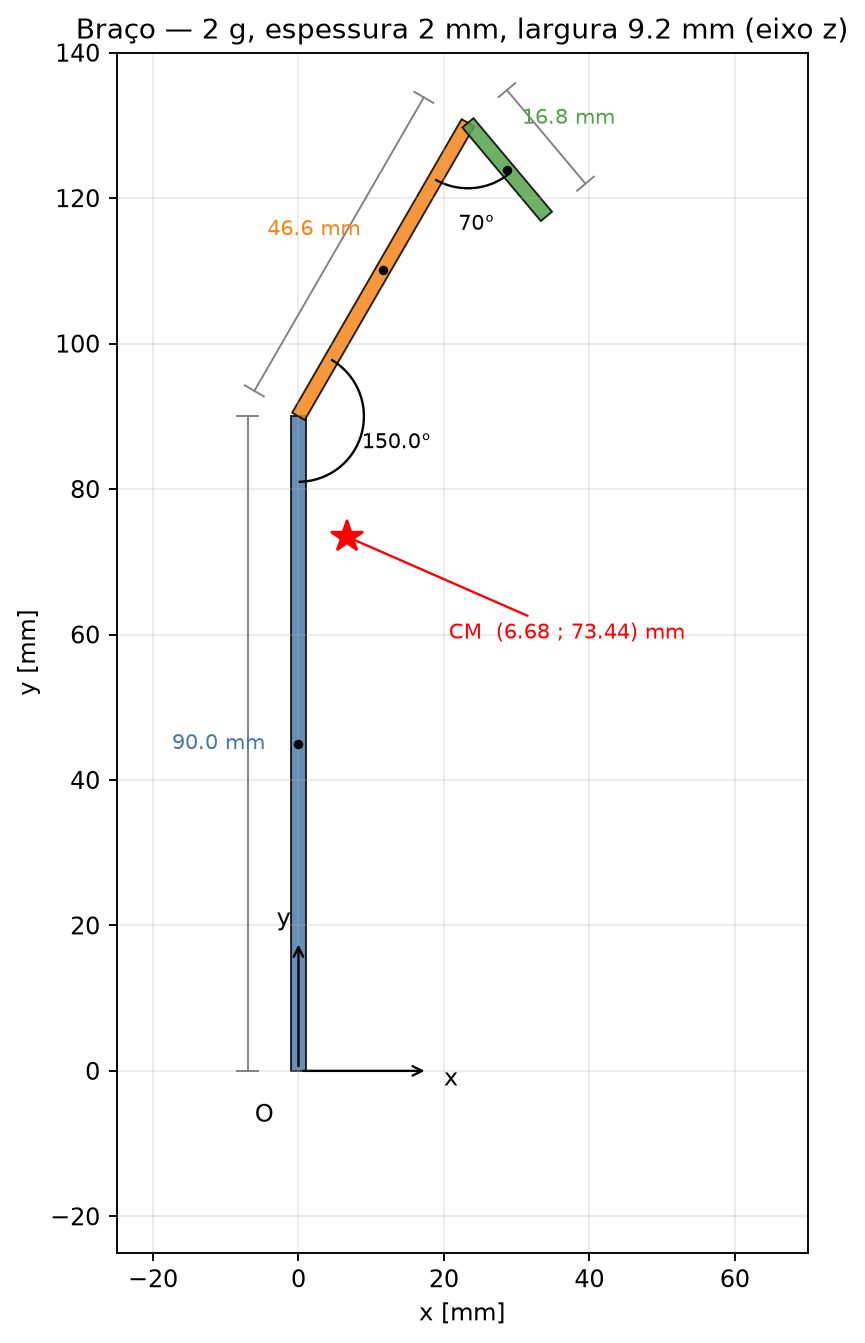
\includegraphics[height=9.5cm]{braco.png}
\caption{\label{fig:braco_modelo}- Modelo do braço (escala real), com cotas, ângulos internos e centro de massa (estrela).}
\end{center}
\end{figure}

\begin{equation*}
\vec{r}_{cm} = (6{,}68; 73{,}44; 0)\ \text{mm}, \qquad [I^*_{\text{braço}}] = \begin{bmatrix}3219{,}0 & -622{,}4 & 0 \\
-622{,}4 & 217{,}9 & 0 \\
0 & 0 & 3408{,}7
\end{bmatrix}\ \text{g}\cdot\text{mm}^2,
\end{equation*}

\noindent com momentos principais de 93,9; 3343,0; 3408,7 g$\cdot$mm$^2$. O produto de inércia $I_{xy}$ não nulo decorre da dobra do braço, e a nulidade de $I_{xz}$ e $I_{yz}$ confirma que o plano da dobra é um plano de simetria de massa.

\subsection{Perna}

A perna é formada por três barras (\ref{fig:perna_modelo}): a haste inferior (44,0 mm), a haste superior inclinada (46,0 mm) e o pé (21,0 mm), com massa total de 1,50 g repartida proporcionalmente ao comprimento (0,59 g, 0,62 g e 0,28 g). O ângulo interno do joelho, medido na fotografia da perna, vale 138,8$^\circ$. O pé não é centrado na haste: a partir do eixo da haste, o calcanhar mede 7,0 mm e o dedão 14,0 mm, de modo que o centro do pé fica deslocado 3,5 mm para a frente. A origem é a extremidade inferior da haste de 44 mm.

\begin{figure}[H]
\begin{center}
 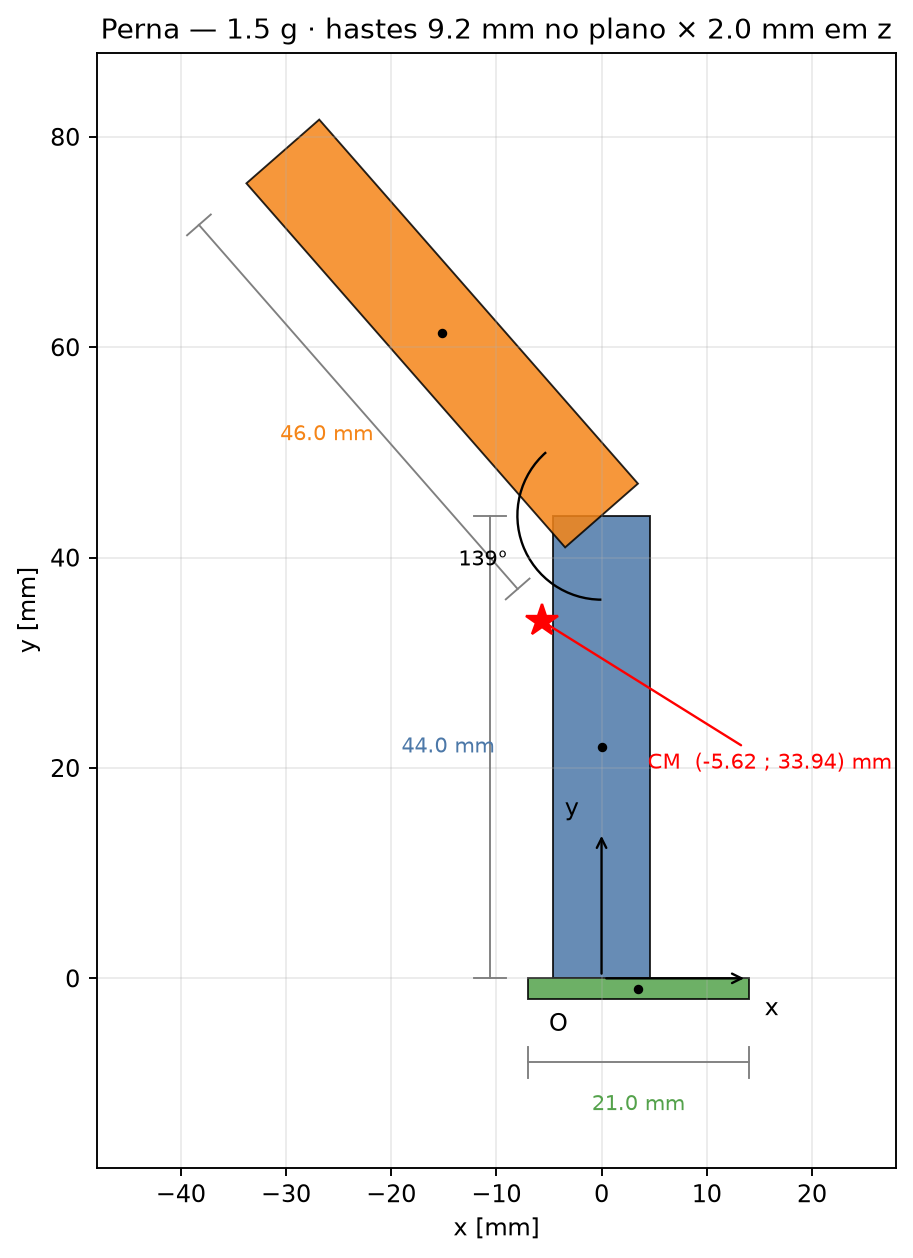
\includegraphics[height=9.5cm]{perna.png}
\caption{\label{fig:perna_modelo}- Modelo da perna (escala real), com calcanhar e dedão.}
\end{center}
\end{figure}

\begin{equation*}
\vec{r}_{cm} = (-5{,}62; 33{,}94; 0)\ \text{mm}, \qquad [I^*_{perna}] = \begin{bmatrix}1059{,}1 & 344{,}6 & 0 \\
344{,}6 & 165{,}9 & 0 \\
0 & 0 & 1220{,}2
\end{bmatrix}\ \text{g}\cdot\text{mm}^2,
\end{equation*}

\noindent com momentos principais de 48,4; 1176,6; 1220,2 g$\cdot$mm$^2$.

\subsection{Ombro (manivela)}

O ombro é a peça que acopla o eixo do motor às alavancas. É formado por uma pilha de três camadas de palito (a inferior com 19,2 mm de comprimento e as duas superiores com 13,0 mm, todas com 9,2 mm de largura e 5,5 mm de altura total), um furo passante de 5,0 mm de diâmetro para o eixo do motor e um pino de 3,5 mm de diâmetro apoiado na camada inferior, cujo eixo dista 9,0 mm do eixo do furo (raio da manivela) e cuja extremidade livre fica a 29,1 mm da face inferior da pilha (\ref{fig:ombro_modelo}). O furo foi tratado como massa negativa, e a massa total de 0,83 g foi distribuída pelo volume. O sistema da peça tem origem no eixo do furo, na face inferior da base, com $z$ ao longo do eixo.

\begin{figure}[H]
\begin{center}
 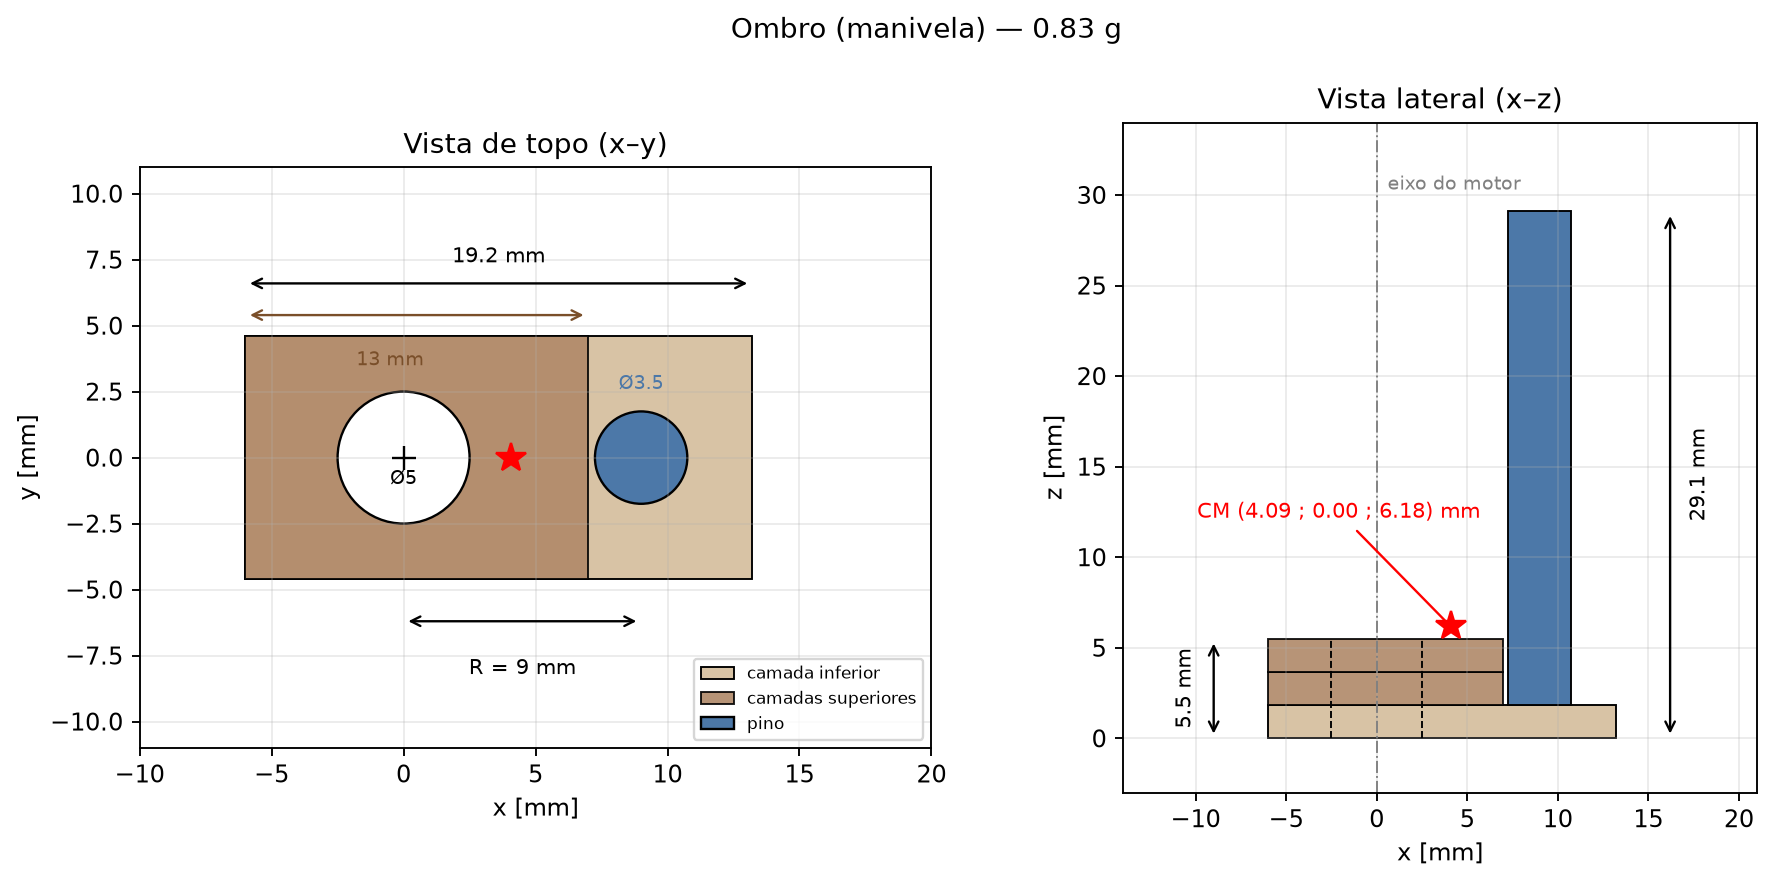
\includegraphics[width=14cm]{ombro.png}
\caption{\label{fig:ombro_modelo}- Modelo do ombro: vistas de topo e lateral, com furo, pino e centro de massa.}
\end{center}
\end{figure}

\begin{equation*}
\vec{r}_{cm} = (4{,}09; 0; 6{,}18)\ \text{mm}, \qquad [I^*_{ombro}] = \begin{bmatrix}49{,}9 & 0 & -13{,}8 \\
0 & 68{,}9 & 0 \\
-13{,}8 & 0 & 28{,}8
\end{bmatrix}\ \text{g}\cdot\text{mm}^2.
\end{equation*}

\noindent O momento de inércia em torno do eixo do motor, obtido por $I_{zz}^* + m\,d^2$, vale $J_{eixo} = 42,7$ g$\cdot$mm$^2$ ($4{,}27\cdot 10^{-8}$ kg$\cdot$m$^2$). O centro de massa fica a 4,1 mm do eixo, o que torna a manivela também uma massa excêntrica.

\subsection{Motor com caixa de redução}

O motor é do tipo com caixa de redução plástica, cujas dimensões foram obtidas do desenho técnico do fabricante (\ref{fig:desenho_motor}): caixa de 22,5 mm $\times$ 31,8 mm $\times$ 18,8 mm, eixo de saída duplo de 5,4 mm de diâmetro (salientes de 8,5 mm e 9,5 mm, totalizando 36,8 mm), comprimento total de 64,2 mm e centro do eixo a 11,2 mm do topo da caixa. O corpo do motor tem 30,0 mm de comprimento e 22,5 mm ao longo do eixo; sua dimensão na outra direção (15,0 mm) não consta do desenho e foi estimada. A massa do conjunto foi medida em 26,6 g, sendo 40\,\% atribuídos à caixa de redução e aos eixos e 60\,\% ao motor, que é mais denso por conter ímãs, bobinas e carcaça metálica. O sistema da peça tem origem no centro do eixo de saída, com $y$ apontando do motor para a caixa. A Figura \ref{fig:motor_modelo} apresenta o modelo sólido do conjunto nas vistas frontal e lateral.

\begin{figure}[H]
\begin{center}
 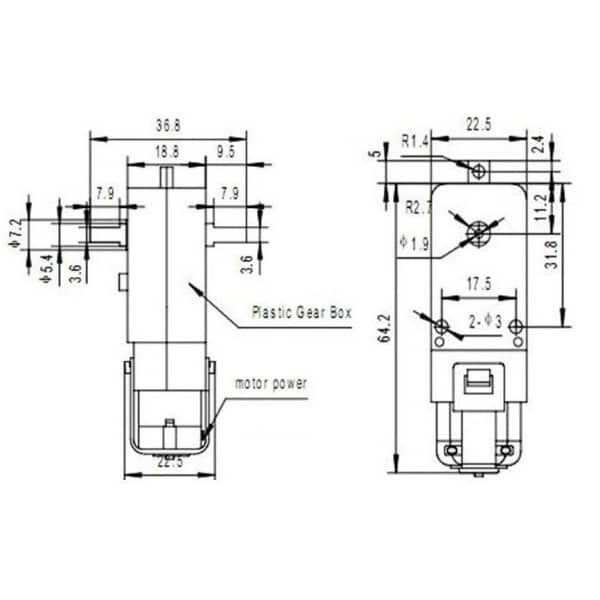
\includegraphics[width=7.5cm]{foto_desenho_motor_dc.jpg}
\caption{\label{fig:desenho_motor}- Desenho técnico do motor com caixa de redução (cotas em mm).}
\end{center}
\end{figure}

\begin{figure}[H]
\begin{center}
 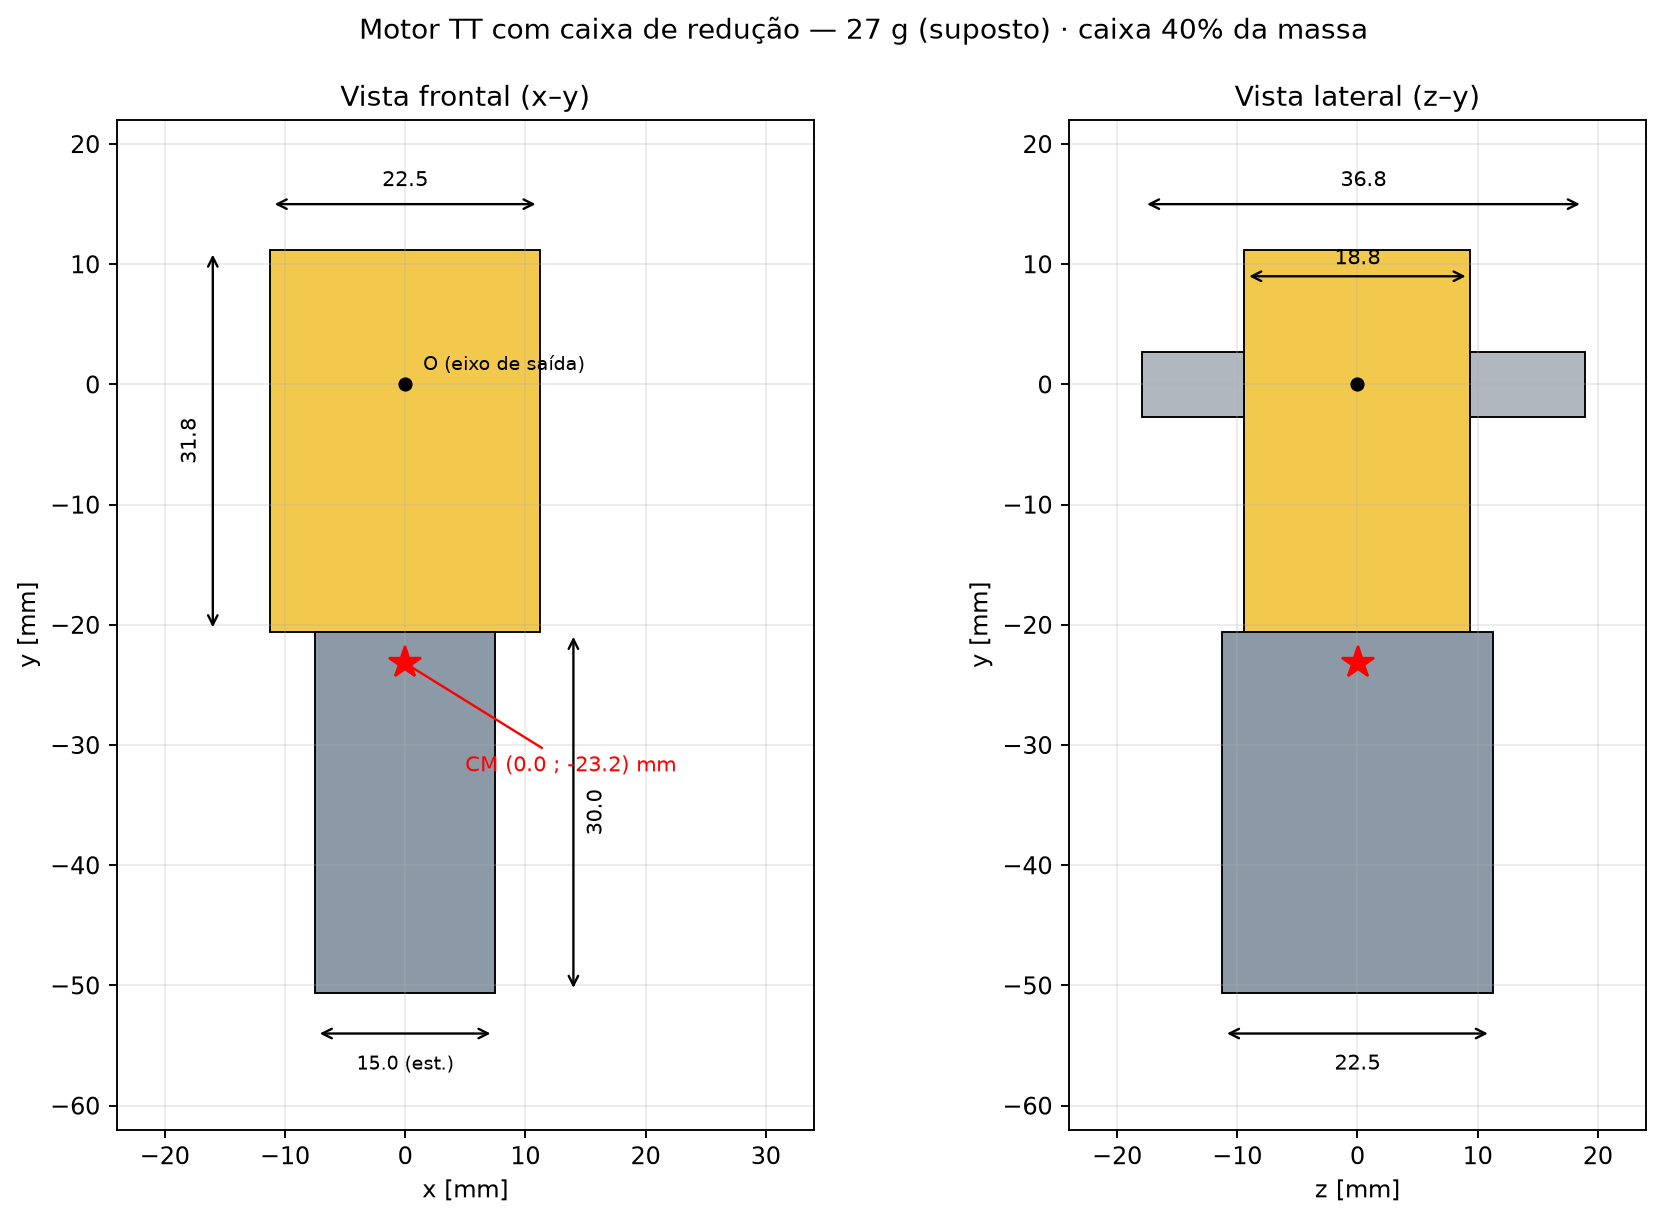
\includegraphics[width=13cm]{motor.png}
\caption{\label{fig:motor_modelo}- Modelo do motor (vistas frontal e lateral).}
\end{center}
\end{figure}

\begin{equation*}
\vec{r}_{cm} = (0; -23{,}18; 0{,}01)\ \text{mm}, \qquad [I^*_{motor}] = \begin{bmatrix}9265{,}9 & 0 & 0 \\
0 & 1776{,}2 & -7{,}5 \\
0 & -7{,}5 & 8960{,}5
\end{bmatrix}\ \text{g}\cdot\text{mm}^2.
\end{equation*}

\subsection{Bateria}

A bateria é um paralelepípedo de 33,55 mm $\times$ 13,9 mm $\times$ 67,7 mm e massa de 67,0 g, o que corresponde a uma densidade média de 2,12 g/cm$^3$, valor coerente com o de uma bateria de lítio. Tratada como sólido homogêneo, seu tensor no centro de massa é diagonal (\ref{fig:bateria_modelo}):

\begin{equation*}
[I^*_{bateria}] = \begin{bmatrix}26680{,}7 & 0 & 0 \\
0 & 31888{,}9 & 0 \\
0 & 0 & 7366{,}7
\end{bmatrix}\ \text{g}\cdot\text{mm}^2.
\end{equation*}

\begin{figure}[H]
\begin{center}
 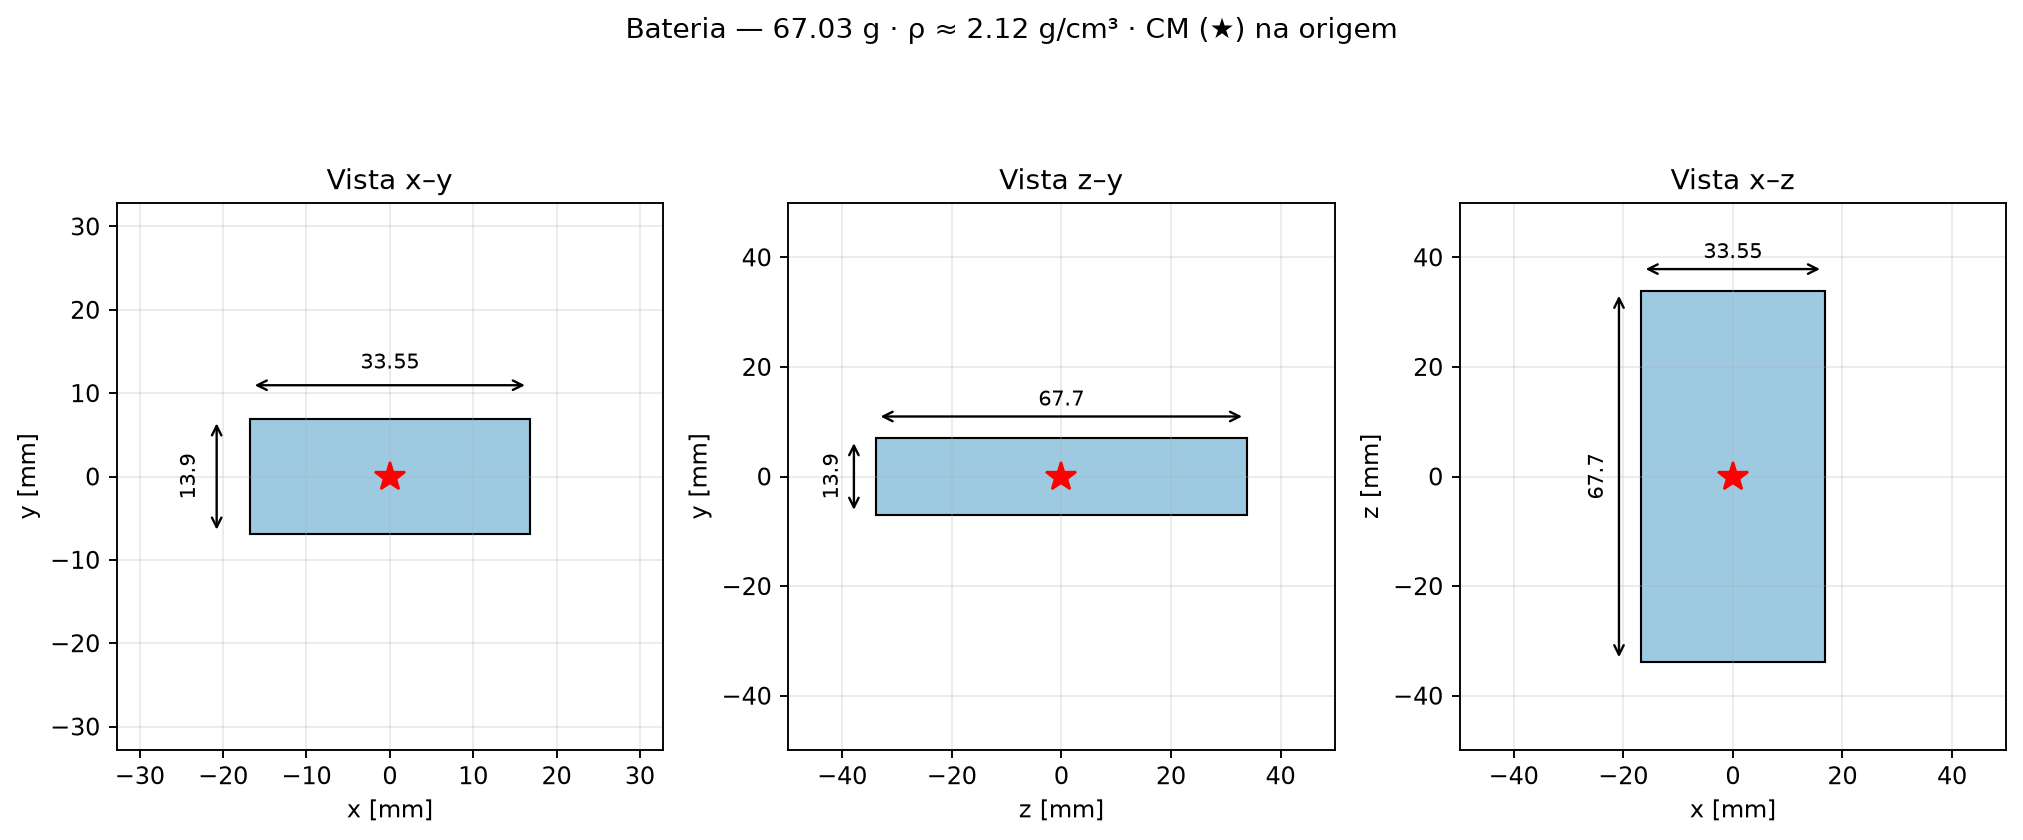
\includegraphics[width=14cm]{bateria.png}
\caption{\label{fig:bateria_modelo}- Modelo da bateria, em três vistas.}
\end{center}
\end{figure}

\subsection{Quadril}

O quadril é uma haste cilíndrica de 3,5 mm de diâmetro e 84,2 mm de comprimento, com massa de 0,81 g. Sua densidade seria de 1,00 g/cm$^3$ se a seção fosse circular e de 0,79 g/cm$^3$ se fosse quadrada, mas a diferença entre as duas hipóteses no momento de inércia transversal é de apenas 0,04\,\%. Com o eixo ao longo de $z$:

\begin{equation*}
[I^*_{quadril}] = \begin{bmatrix}479{,}2 & 0 & 0 \\
0 & 479{,}2 & 0 \\
0 & 0 & 1{,}2
\end{bmatrix}\ \text{g}\cdot\text{mm}^2,
\end{equation*}

\noindent ou seja, a haste comporta-se como uma barra fina ($I \approx mL^2/12$ nas direções transversais).

\section{Montagem do Robô Completo}
\label{sec:montagem}

A posição relativa das peças foi definida a partir da vista frontal do protótipo (\ref{fig:frontal}), que fornece duas cotas: 42 mm entre os palitos dos dois membros e 45,5 mm entre o eixo do motor (nível dos pinos das manivelas) e o eixo do quadril. Adotou-se:

\begin{itemize}
  \item membros nos planos $z=\pm 22$ mm (folga de 42 mm mais 2 mm de espessura) e quadril em $y=-45{,}5$ mm;
  \item manivelas montadas nos dois lados da caixa, com os pinos defasados de 180$^\circ$, de modo que, quando um braço vai para trás, o outro vai para a frente;
  \item braços como corpos rígidos que giram em torno do eixo do quadril e passam pelos pinos das manivelas (Seção \ref{sec:alavancas}), com extremidade inferior livre em $y=-66$ mm;
  \item pernas penduradas do eixo do quadril, com o furo do quadril 4,6 mm abaixo da extremidade superior da perna (estimado), dedão voltado para a frente e calcanhar atrás;
  \item bateria nas costas do robô, encostada na face traseira da caixa de redução e centrada em relação ao conjunto motor--caixa, com o lado de 67,7 mm na vertical.
\end{itemize}

\begin{figure}[H]
\begin{center}
 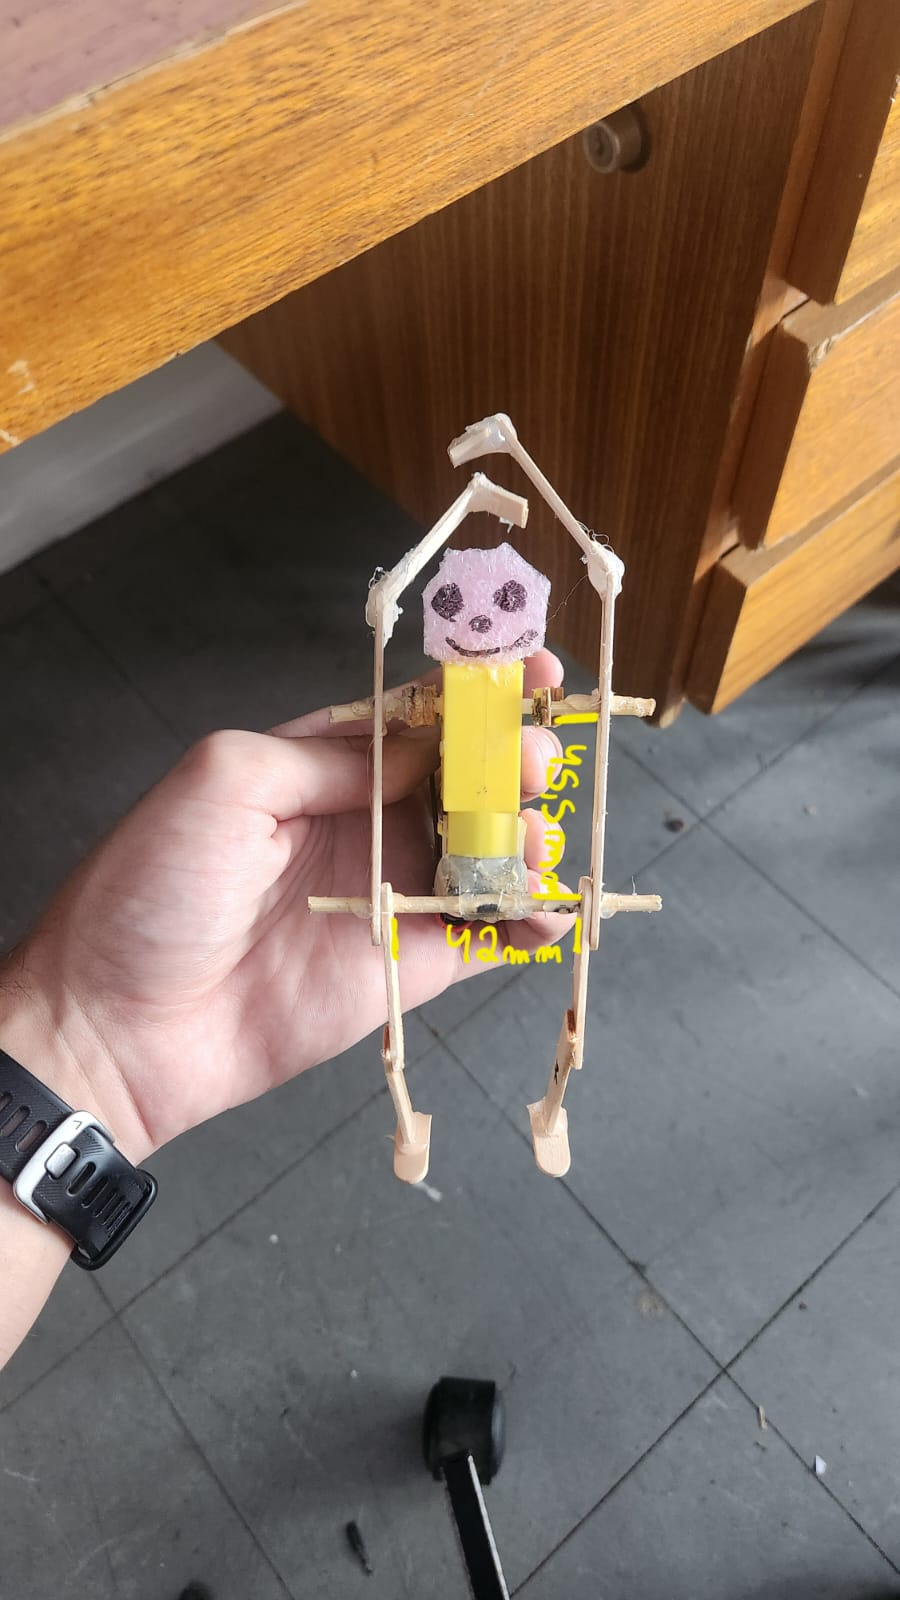
\includegraphics[height=10cm]{foto_robo_montado.jpeg}
\caption{\label{fig:frontal}- Vista frontal do protótipo montado, com as cotas de 42 mm e 45,5 mm.}
\end{center}
\end{figure}

A \ref{fig:robo_montado} mostra a montagem nas vistas frontal e lateral, para a posição da manivela $\psi = 0^\circ$ (pinos no nível do eixo do motor), e a \ref{tab:instancias} lista a massa e o centro de massa de cada peça no sistema do corpo.

\begin{figure}[H]
\begin{center}
 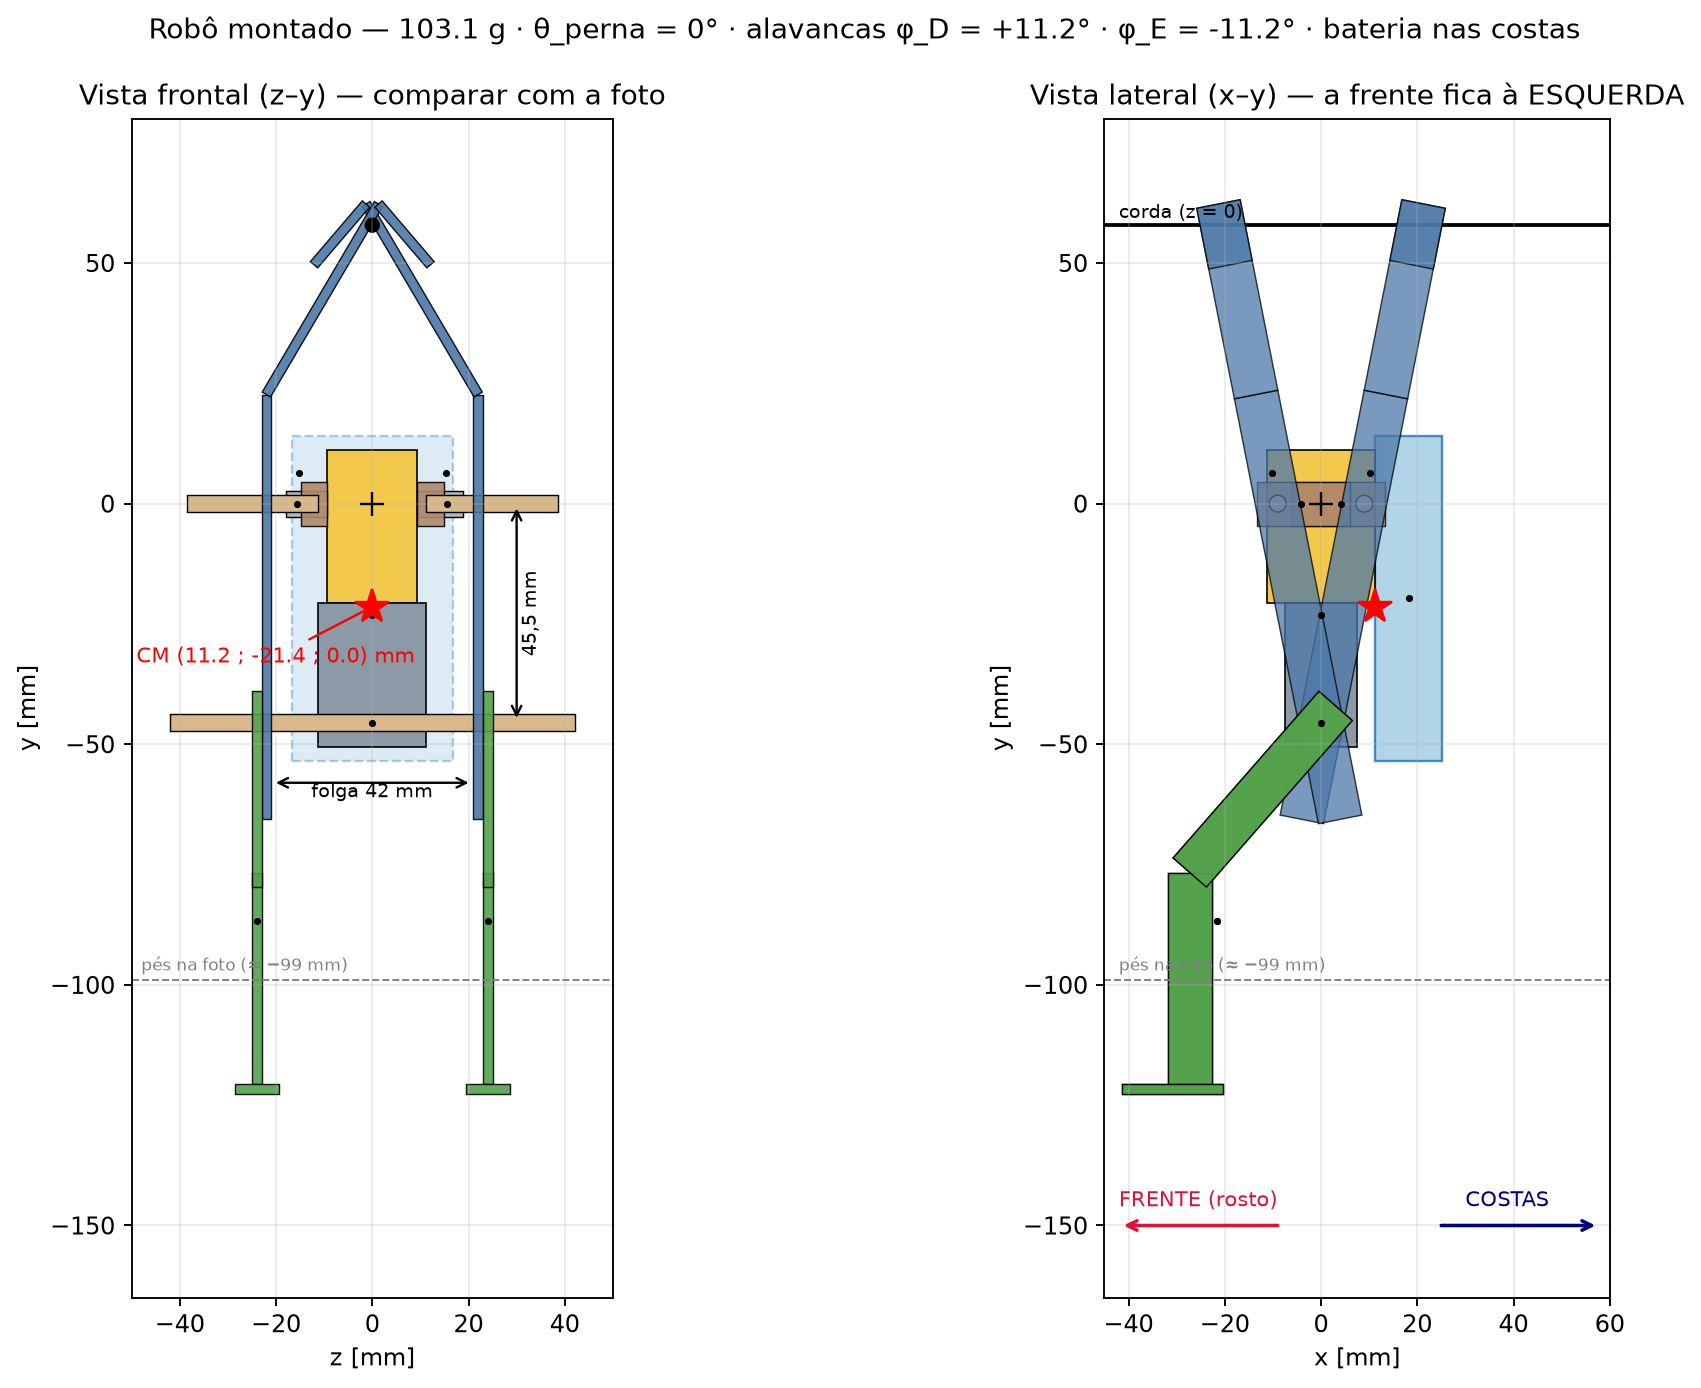
\includegraphics[width=15cm]{robo.png}
\caption{\label{fig:robo_montado}- Robô montado, nas vistas frontal e lateral (a frente fica à esquerda na vista lateral).}
\end{center}
\end{figure}

\begin{table}[H]
\centering
\caption{\label{tab:instancias}- Massa e centro de massa de cada peça no sistema do corpo (posição $\psi=0^\circ$).}
\vspace*{.1cm}
\begin{tabular}{|l|c|c|c|c|}
\hline
\textbf{Peça} & \textbf{Massa (g)} & \textbf{$x_{cm}$ (mm)} & \textbf{$y_{cm}$ (mm)} & \textbf{$z_{cm}$ (mm)} \\
\hline
Motor com caixa de redução & 26,60 & 0,00 & $-$23,18 & 0,01 \\
\hline
Quadril & 0,81 & 0,00 & $-$45,50 & 0,00 \\
\hline
Ombro D & 0,83 & 4,09 & 0,00 & 15,58 \\
\hline
Ombro E & 0,83 & $-$4,09 & 0,00 & $-$15,58 \\
\hline
Braço D & 2,00 & 10,27 & 6,44 & 15,32 \\
\hline
Braço E & 2,00 & $-$10,27 & 6,44 & $-$15,32 \\
\hline
Perna D & 1,50 & $-$21,65 & $-$86,71 & 24,00 \\
\hline
Perna E & 1,50 & $-$21,65 & $-$86,71 & $-$24,00 \\
\hline
Bateria & 67,03 & 18,20 & $-$19,70 & 0,00 \\
\hline
\end{tabular}
\end{table}

O robô completo, com a bateria, tem massa de 103,1 g e centro de massa em (11{,}20; -21{,}42; 0) mm, ou seja, 21,4 mm abaixo do eixo do motor e 11,2 mm atrás dele. O tensor de inércia em torno do centro de massa e os momentos principais são:

\begin{equation*}
[I^*_{\text{robô}}] = \begin{bmatrix}70904{,}3 & -7029{,}3 & -517{,}6 \\
-7029{,}3 & 24957{,}8 & -6{,}9 \\
-517{,}6 & -6{,}9 & 73105{,}0
\end{bmatrix}\ \text{g}\cdot\text{mm}^2, \qquad \text{principais: } 23906; 71761; 73299\ \text{g}\cdot\text{mm}^2.
\end{equation*}

\noindent Em torno do centro do eixo de saída do motor (ponto $O$), o tensor vale

\begin{equation*}
[I_{O,\text{robô}}] = \begin{bmatrix}118210 & 17711 & -521 \\
17711 & 37897 & 0 \\
-521 & 0 & 133349
\end{bmatrix}\ \text{g}\cdot\text{mm}^2.
\end{equation*}

\noindent O tensor depende da posição da manivela, pois os braços inclinam-se alternadamente; os valores acima correspondem a $\psi=0^\circ$. O motor e a bateria respondem por 91\,\% da massa, o que explica a posição baixa do centro de massa e o fato de os produtos de inércia serem pequenos frente aos momentos principais.

\section{Momentos de Inércia dos Corpos Móveis em Torno dos Pivôs}
\label{sec:corpos_moveis}

Como o movimento ocorre no plano $x$--$y$, a dinâmica depende apenas do momento de inércia em torno de eixos paralelos a $z$. Esse momento independe do ângulo de rotação em torno de $z$ e foi calculado para cada corpo móvel em torno do seu pivô por $I_{piv\hat{o}} = I^*_{zz} + m\,d^2$ (Seção \ref{sec:composicao}). A \ref{tab:corpos} reúne os resultados, que são os dados de entrada do modelo dinâmico do Capítulo \ref{chapter:modelo}.

\begin{table}[H]
\centering
\caption{\label{tab:corpos}- Corpos móveis do modelo dinâmico: massa, momento de inércia no centro de massa e em torno do pivô.}
\vspace*{.1cm}
\small
\begin{tabular}{|l|c|c|c|c|}
\hline
\textbf{Corpo} & \textbf{Massa (g)} & \textbf{$I^*_{zz}$ (g$\cdot$mm$^2$)} & \textbf{Pivô} & \textbf{$I_{piv\hat{o}}$ (g$\cdot$mm$^2$)} \\
\hline
Manivela D & 0,83 & 28,8 & eixo do motor & 42,7 \\
\hline
Manivela E & 0,83 & 28,8 & eixo do motor & 42,7 \\
\hline
Alavanca D (braço) & 2,00 & 3219,0 & eixo do quadril & 8825,0 \\
\hline
Alavanca E (braço) & 2,00 & 3219,0 & eixo do quadril & 8825,0 \\
\hline
Perna D & 1,50 & 1220,2 & eixo do quadril & 4471,2 \\
\hline
Perna E & 1,50 & 1220,2 & eixo do quadril & 4471,2 \\
\hline
Chassi (motor, quadril e bateria) & 94,44 & 42812 & --- & --- \\
\hline
\end{tabular}
\end{table}

O chassi reúne o motor com a caixa de redução, o quadril e a bateria e tem centro de massa em (12{,}92; -20{,}90; 0) mm. As alavancas têm inércia em torno do quadril 2,7 vezes maior que a própria ($I_{piv\hat{o}}/I^*_{zz}$) porque seu centro de massa fica a cerca de 52 mm do eixo; nas pernas, essa razão é de 3,7.
